\documentclass[11pt]{article}

% ---------------------------------------------------------------------------
% Atomic and molecular calculations with explicitly correlated Gaussians:
% an efficient open implementation in Julia.
%
% Draft for circulation to S. Bubin and K. L. Sharkey; potential arXiv submission.
% Author: Alain Chancé (MOLKET SAS).
% ---------------------------------------------------------------------------

\usepackage[utf8]{inputenc}
\usepackage[T1]{fontenc}
\usepackage{amsmath,amssymb,amsfonts}
\usepackage{bm}
\usepackage{graphicx}
\usepackage{booktabs}
\usepackage{array}
\usepackage{geometry}
\geometry{margin=1in}
\usepackage[hidelinks]{hyperref}
\usepackage{listings}
\usepackage{xcolor}
\usepackage{lmodern}
\usepackage{orcidlink}

\lstset{basicstyle=\ttfamily\small,breaklines=true,frame=single,
        backgroundcolor=\color{gray!8},columns=fullflexible}

\newcommand{\rvec}{\mathbf{r}}
\newcommand{\vech}{\operatorname{vech}}
\newcommand{\vecop}{\operatorname{vec}}
\newcommand{\Hcal}{\hat{H}}
\newcommand{\Ycal}{\hat{Y}}

\title{Atomic and Molecular Calculations with Explicitly Correlated
Gaussians: An Efficient Open Implementation in Julia}

\author{Alain Chanc\'e\thanks{MOLKET SAS, \texttt{alain.chance@gmail.com}.},
\orcidlink{0009-0004-3619-2267}}

\date{\today}

\begin{document}
\maketitle

\begin{abstract}
We present \texttt{ECG\_Julia}, an open, modular implementation in the Julia
programming language of the variational method of explicitly correlated
Gaussians (ECGs) for non-relativistic, finite-nuclear-mass atomic and
molecular bound-state calculations. The code follows the formalism reviewed
by Bubin, Pavanello, Tung, Sharkey and Adamowicz~\cite{Bubin2013} and the
matrix-element algebra of Kinghorn~\cite{Kinghorn1996}, Bubin and
Adamowicz~\cite{Bubin2008}, and Sharkey and Adamowicz~\cite{Sharkey2014}.
Four basis-function families are supported: two real correlated Gaussians for
$L=0$ states (\texttt{RGL0}), two complex correlated Gaussians for $L=0$
states (\texttt{CGL0}), the $L=0$ nitrogen basis with a cubic angular
prefactor (\texttt{N\_Pvec}/\texttt{N\_C\_Pvec}), and two real correlated
Gaussians for $L=1$ states (\texttt{RGL1}). The package combines a
JSON-driven run configuration, an automatically-differentiated analytic
energy gradient, a symmetry-term truncation/ramp scheme for accelerating
the nonlinear optimization of large permutation operators, and an optional
text-file bridge to the reference Fortran program \textsc{atom-mol-nonBO}.
The primary contribution is the implementation itself---its modular software
architecture, its forward-mode automatic-differentiation design, and its
on-the-fly construction and handling of the permutational-symmetry
operator---released as open-source software so that it can be inspected,
reused and extended. To verify correctness across all four models we
reproduce published ground-state energies for $\mathrm{HD^+}$,
$\mathrm{D_3^+}$, $\mathrm{H_3^+}$, $^9\mathrm{Be}$, $\mathrm{He}$, $^7\mathrm{Li}$,
$^{14}\mathrm{N}$, and the positronium molecule $\mathrm{Ps_2}$; these
calculations serve as validation of the code rather than as new or
best-available reference data.
\end{abstract}

\tableofcontents

% =====================================================================
\section*{Executive summary}
\addcontentsline{toc}{section}{Executive summary}

Explicitly correlated Gaussian (ECG) basis functions provide some of the most
accurate non-relativistic energies available for small atoms and molecules
because the interparticle distances enter the basis explicitly, and because
the Born--Oppenheimer separation can be dropped entirely (all particles,
nuclei and electrons, are treated on the same footing)~\cite{Bubin2013}. The
price is a demanding nonlinear optimization of the Gaussian exponent matrices
and an expensive permutational-symmetry projection.

This work re-implements the established ECG methodology in Julia, with three
aims: (i) a clean, configuration-driven, reproducible code base in which each
physical model is a self-contained matrix-element module; (ii) a faster
nonlinear optimization, obtained from an exact analytic energy gradient
generated by forward-mode automatic differentiation and from a multi-fidelity
truncation/ramp of the symmetry operator; and (iii) interoperability with the
reference Fortran program \textsc{atom-mol-nonBO} through a plain text-file
interface, so that results can be cross-checked. The deliverable is therefore
the open implementation itself---a reusable, extensible code base for ECG
calculations---of which the benchmark energies reported below are a
verification rather than the end product. Section~\ref{sec:overview}
summarizes the ECG formalism and the four supported models; Section~\ref{sec:impl}
describes the Julia implementation; Section~\ref{sec:results} verifies the
implementation against published energies; Section~\ref{sec:conclusion} concludes. Appendices~A--C give
the Hamiltonian and permutational symmetry, the solution of the secular
equation (including the analytic/automatic-differentiation gradient), and the
$\vecop$/$\vech$ matrix operators.

% =====================================================================
\section{Overview of atomic and molecular calculations with explicitly correlated Gaussians}
\label{sec:overview}

For the authoritative and comprehensive account of the method we refer the
reader to Bubin, Pavanello, Tung, Sharkey and Adamowicz, \emph{Born--Oppenheimer
and Non-Born--Oppenheimer, Atomic and Molecular Calculations with Explicitly
Correlated Gaussians}, Chem.\ Rev.\ \textbf{113}, 36--79
(2013)~\cite{Bubin2013}. The present section recalls only what is needed to
define the four models implemented in \texttt{ECG\_Julia}.

For an $n$-pseudoparticle system (after separation of the center-of-mass
motion) with internal Cartesian coordinates collected in the $3n$-vector
$\rvec$, the variational wave function is a linear combination of
symmetry-projected ECGs,
\begin{equation}
\psi(\rvec)=\sum_{k=1}^{K} c_k\, \Ycal\, \phi_k(\rvec),
\end{equation}
where $\Ycal$ is the permutational-symmetry projector (a linear combination of
permutation operators; Appendix~A), the $c_k$ are linear variational
coefficients, and the $\phi_k$ are correlated Gaussians whose exponent matrices
contain the nonlinear variational parameters. Minimizing the Rayleigh quotient
with respect to the $c_k$ leads to the generalized symmetric/Hermitian
eigenproblem
\begin{equation}
(\mathbf{H}-\varepsilon\,\mathbf{S})\,\mathbf{c}=\mathbf{0},
\qquad
\mathrm{H}_{kl}=\big\langle \phi_k \big| \Hcal\, \Ycal^{\dagger}\Ycal \big| \phi_l \big\rangle,
\qquad
\mathrm{S}_{kl}=\big\langle \phi_k \big| \Ycal^{\dagger}\Ycal \big| \phi_l \big\rangle,
\end{equation}
solved repeatedly inside an outer optimization of the nonlinear parameters
(Appendix~B). The four models differ in the form of $\phi_k$.

% ---------------------------------------------------------------
\subsection{Two real correlated Gaussians for states with rotation quantum number \texorpdfstring{$L=0$}{L=0} (module \texttt{RGL0})}
\label{sec:rgl0}

For $L=0$ states (all particles in $s$-states) the spatial basis function has
only a radial exponential part,
\begin{equation}
\phi_k(\rvec)=\exp\!\left[-\rvec'\,\overline{\mathbf{A}}_k\,\rvec\right],
\qquad k=1,\dots,K,
\end{equation}
where the prime denotes transposition. The $3n\times 3n$ real symmetric
exponent matrix factorizes as $\overline{\mathbf{A}}_k=A_k\otimes I_3$, with
$I_3$ the $3\times 3$ identity, $\otimes$ the Kronecker product, and $A_k$ an
$n\times n$ symmetric matrix. To guarantee a positive-definite quadratic form,
$A_k$ is held in Cholesky-factored form $A_k=L_kL_k'$ with $L_k$ an $n\times n$
lower-triangular matrix, so that
\begin{equation}
\phi_k(\rvec)=\exp\!\left[-\rvec'\,(L_kL_k'\otimes I_3)\,\rvec\right].
\end{equation}
The nonlinear variational parameters are the lower-triangular elements of the
$L_k$ (the $\vech L_k$; Appendix~C). This is the \texttt{ECG\_Matelem\_RGL0}
module.

% ---------------------------------------------------------------
\subsection{Two complex correlated Gaussians for states with rotation quantum number \texorpdfstring{$L=0$}{L=0} (module \texttt{CGL0})}
\label{sec:cgl0}

Complex exponent matrices add variational flexibility~\cite{Bubin2013}. The
basis function reads
\begin{equation}
\phi_k(\rvec)=\exp\!\left[-\rvec'\,\overline{\mathbf{C}}_k\,\rvec\right]
=\exp\!\left[-\rvec'\big(\overline{\mathbf{A}}_k+\mathrm{i}\,\overline{\mathbf{B}}_k\big)\rvec\right],
\end{equation}
where $\overline{\mathbf{A}}_k=A_k\otimes I_3$ and
$\overline{\mathbf{B}}_k=B_k\otimes I_3$ with $A_k$, $B_k$ real symmetric
$n\times n$ matrices, $A_k=L_kL_k'$ as before. This is the
\texttt{ECG\_Matelem\_CGL0} module.

% ---------------------------------------------------------------
\subsubsection{Nitrogen with rotation quantum number \texorpdfstring{$L=0$}{L=0} (modules \texttt{N\_Pvec}, \texttt{N\_matr}, \texttt{N\_C\_Pvec})}
\label{sec:nitrogen}

For the $^4S$ ground state of nitrogen, with three $p$-electrons coupled to
$L=0$, $M=0$, the basis function carries a cubic angular prefactor
\cite{Sharkey2014}:
\begin{equation}
\begin{aligned}
\psi_f=&\Big\{\big(x_{j_f}y_{i_f}-x_{i_f}y_{j_f}\big)z_{k_f}
+\big(x_{i_f}y_{k_f}-x_{k_f}y_{i_f}\big)z_{j_f}\\
&+\big(x_{k_f}y_{j_f}-x_{j_f}y_{k_f}\big)z_{i_f}\Big\}
\exp\!\left[-\rvec'\mathbf{A}_f\rvec\right].
\end{aligned}
\end{equation}
This prefactor has six unique terms, so each Hamiltonian or overlap matrix
element requires the evaluation of $36$ elemental integrals.

\paragraph{Permutational symmetry.}
Symmetry adaptation is enforced by projecting with the Young operator $\Ycal$
(Appendix~A):
\begin{equation}
\psi_k=\Ycal\,\Phi_k=\sum_{P}\chi_P\, r_1^{m_k}\,
\exp\!\left[-\rvec'\big(\tau_P' L_kL_k'\tau_P\otimes I_3\big)\rvec\right],
\end{equation}
the sum running over permutations of identical-particle labels, with
permutation matrices $\tau_P$. For nitrogen the complete operator
$\Ycal^{\dagger}\Ycal$ has $n!=7!=5040$ terms.

\paragraph{Overlap, potential and kinetic matrix elements.}
With $A_{fg}$ the combined exponent matrix and
$\eta_x\equiv (A_{fg}^{-1})_{(x_f,P\vecop(x_g))}$ (and analogously for $y,z$),
the overlap is~\cite{Sharkey2014}
\begin{equation}
\langle\phi_f|\phi_g\rangle=\tfrac{1}{8}\pi^{3n/2}\,|A_{fg}|^{-3/2}\,
\eta_x\eta_y\eta_z,
\end{equation}
the electron--nucleus / electron--electron potential element is
\begin{equation}
\begin{aligned}
\Big\langle\phi_f\Big|\tfrac{1}{r_{i'j'}}\Big|\phi_g\Big\rangle=&
\tfrac{1}{4}\pi^{(3n-1)/2}\,|A_{fg}|^{-3/2}\,\lambda^{-1/2}
\Big\{\eta_x\eta_y\eta_z
-\tfrac{\lambda^{-1}}{3}\big(\eta_x\eta_y\eta_{zJ}+\eta_x\eta_{yJ}\eta_z+\eta_{xJ}\eta_y\eta_z\big)\\
&+\tfrac{\lambda^{-2}}{5}\big(\eta_x\eta_{yJ}\eta_{zJ}+\eta_{xJ}\eta_y\eta_{zJ}+\eta_{xJ}\eta_{yJ}\eta_z\big)
-\tfrac{\lambda^{-3}}{7}\,\eta_{xJ}\eta_{yJ}\eta_{zJ}\Big\},
\end{aligned}
\end{equation}
and the kinetic element is
\begin{equation}
\begin{aligned}
\langle\nabla_\rvec\phi_f|\mathbf{M}|\nabla_\rvec\phi_g\rangle=&
\tfrac{1}{4}\pi^{3n/2}\,|A_{fg}|^{-3/2}\Big\{3\tau\,\eta_x\eta_y\eta_z\\
&+\big(M_{(x_f,P\vecop(x_g))}+2\tau_x-(A_{fg}^{-1}A_fM)_{(x_f,P\vecop(x_g))}-(MA_gA_{fg}^{-1})_{(x_f,P\vecop(x_g))}\big)\eta_y\eta_z\\
&+(x\!\to\!y)\,\eta_x\eta_z+(x\!\to\!z)\,\eta_x\eta_y\Big\}.
\end{aligned}
\end{equation}
Three modules implement these elements: \texttt{N\_Pvec} and \texttt{N\_matr}
(real Gaussians) and \texttt{N\_C\_Pvec} (complex). With the $36$ elemental
integrals carried by each of the $n!=5040$ permutation terms, evaluating a single
nitrogen Hamiltonian or overlap matrix element requires the elemental-integral
formula to be applied $180{,}240$ times~\cite{Sharkey2014}, so minimizing the work
per permutation is essential. Following the permutational-symmetry scheme of
Sharkey and Adamowicz~\cite{Sharkey2014} (Sec.~IV), the \texttt{Pvec} variants
avoid forming permutation-matrix products altogether: the forwards-direction
permutation $(P_g v = v'P_g')$ is stored in the first half and the
backwards-direction permutation $(P_g'v = vP_g')$ in the second half of a
$2n$-component index vector $\mathrm{pvec}$ (Appendix~C), so a permuted
width-matrix element is obtained by an index gather,
\begin{equation}
(P_g A P_g')_{(s,t)}=A_{(\mathrm{pvec}(s),\,\mathrm{pvec}(t))},\qquad
(P_g' A P_g)_{(s,t)}=A_{(\mathrm{pvec}(s+n),\,\mathrm{pvec}(t+n))},
\end{equation}
rather than by multiplying matrices --- ``as long as we know the order of the
particles, we know the order of the permuted matrix''~\cite{Sharkey2014}. This
reduces forming $P_g'A_gP_g$ from $2n^3$ to $n^2$ operations (for nitrogen,
$686\to49$) and permuting a $3n$-vector from $(3n)^2$ to $n$ ($441\to7$) --- the
principal per-permutation saving that \texttt{ECG\_Julia} inherits.

% ---------------------------------------------------------------
\subsection{Two real correlated Gaussians for states with rotation quantum number \texorpdfstring{$L=1$}{L=1} (module \texttt{RGL1})}
\label{sec:rgl1}

For $L=1$ states (one particle in a $p$-state, the rest in $s$-states) the
basis function carries a single linear prefactor~\cite{Bubin2008}:
\begin{equation}
\phi_k(\rvec)=z_{m_k}\,\exp\!\left[-\rvec'\,\overline{\mathbf{A}}_k\,\rvec\right]
=z_{m_k}\,\exp\!\left[-\rvec'\,(L_kL_k'\otimes I_3)\,\rvec\right],
\end{equation}
where $m_k$ is an integer index depending on $k$. The energy and energy-gradient
matrix elements for $N$-particle $L=1$ complex Gaussians are those of Bubin and
Adamowicz~\cite{Bubin2008}. This is the \texttt{ECG\_Matelem\_RGL1} module; we
use it below for the ground state of the positronium molecule $\mathrm{Ps_2}$
in the $L=1$, negative-parity state.

% =====================================================================
\section{An efficient implementation in Julia}
\label{sec:impl}

\texttt{ECG\_Julia} is organized as a small set of modules, and rests on three
design choices that together constitute the contribution of this work: a
\emph{modular software architecture} in which each physical model is a
self-contained matrix-element module behind a single uniform interface; a
\emph{generic-programming / automatic-differentiation design} that yields exact
analytic energy gradients without hand-coded derivatives; and an
\emph{on-the-fly construction of the permutational-symmetry operator} from a
human-readable Young-operator string. The Julia
language~\cite{Bezanson2017} provides compiled performance with a high-level,
generic programming model; the latter is essential to the
automatic-differentiation gradient described below. We describe each module in
turn, grouping the discussion under these three themes.

\paragraph{\texttt{ECG\_Param}.}
Defines the run parameters and the default-parameter structure \texttt{param0}
(an \texttt{Init\_param} instance): system size, basis size, target energy,
optimization controls, and the model selector \texttt{MatElem\_method}
($\in\{$\texttt{RGL0}, \texttt{CGL0}, \texttt{RGL1}, \texttt{N\_Pvec},
\texttt{N\_matr}, \texttt{N\_C\_Pvec}$\}$). Recent fields control the
optimization accelerators: \texttt{coeff\_threshold} and \texttt{coeff\_ramp\_tol}
(symmetry-term truncation and ramp), \texttt{analytic\_grad} (analytic energy
gradient), and the trial-generation controls
\texttt{gen\_NonlinParam}, \texttt{RG\_p1}, \texttt{RG\_s1}, \texttt{RG\_s2}.

\paragraph{\texttt{ECG\_Config}.}
Reconstructs an entire run from a single JSON file (\texttt{ecg\_config.json})
with three sections: \texttt{setup} (the module and data files copied into the
working directory, and stale files removed, using native-Julia file operations),
\texttt{ECG\_Param} (module-level settings), and \texttt{param0} (fields of the
\texttt{Init\_param} instance). This replaces ad-hoc post-\texttt{include}
mutation of globals and makes runs reproducible and machine-writable.

\paragraph{\texttt{ECG\_Init}.}
Initializes the data structures, reduced-mass and charge data, the
transposition matrices, and the symmetry ($Y$ and $Y^{\dagger}Y$) operators.
The operators are read from reference files when present, and otherwise
computed on the fly by the module \texttt{SymmetryOperators} directly from the
Young-operator string (e.g.\ \verb|(1+P12)(1-P23)|) and the particle count.
The module also generates the Basis-Function Prefactor Index (BFPI) table for
the $L=0$ atomic prefactors and defines \texttt{set\_parvec}, which assembles
the $36$-row index array consumed by the nitrogen matrix-element kernels.

\paragraph{\texttt{ECG}.}
Assembles the Hamiltonian and overlap matrices (\texttt{compute\_H\_S}), solves
the secular equation (\texttt{solve\_sec}, with a Bunch--Kaufman/inverse-iteration
path \texttt{GSEPIIS} and a generalized-eigensolver path), generates trial
nonlinear parameters (\texttt{stoch\_nlp}), performs cyclic nonlinear
optimization (\texttt{optim\_nlp}, built on \texttt{Optim.jl}), and orchestrates
the action list of a run (\texttt{do\_action}). It includes the relevant
\texttt{ECG\_Matelem} module at load time according to \texttt{MatElem\_method}.

Two accelerators are implemented here. First, a \emph{symmetry-term
truncation and ramp}: during the inner BFGS search, $Y^{\dagger}Y$ terms whose
coefficient magnitude falls below \texttt{coeff\_threshold} are skipped, giving
a cheaper partially-symmetrized surface, while every accepted or reported
energy is recomputed with the full operator; an automatic ramp lowers the
threshold tier by tier (eventually to the full operator) as the per-cycle
improvement decays. For nitrogen, whose $5040$-term operator has coefficient
magnitudes in $\{96,192,960\}$, this concentrates early effort on the $240$
dominant terms. Second, an \emph{analytic energy gradient} (Appendix~B): when
\texttt{analytic\_grad} is set, \texttt{optim\_nlp} passes
\texttt{loss\_grad!}\ to the optimizer instead of relying on finite
differences.

\paragraph{\texttt{ECG\_Fortran}.}
Groups the functions that drive and read back the reference Fortran program
\textsc{atom-mol-nonBO}~\cite{ATOMMOLnonBO} through a text-file interface only:
parameters and matrices are exchanged through plain files and the executable is
launched as a subprocess. This enables independent cross-checks of the Julia
energies.

\paragraph{\texttt{ECG\_Matelem} family.}
Each model is a self-contained matrix-element module named
\texttt{ECG\_Matelem\_<Model>} (e.g.\ \texttt{ECG\_Matelem\_CGL0},
\texttt{ECG\_Matelem\_N\_Pvec}), included by \texttt{ECG} at load time according
to \texttt{MatElem\_method}. Each exposes a single \texttt{MatrixElements}
function that returns the normalized $\mathrm{H}_{kl}$, $\mathrm{S}_{kl}$, and
(optionally) their derivatives $\mathrm{Dk}$, $\mathrm{Dl}$ with respect to the
nonlinear parameters. For the nitrogen modules the derivatives are obtained by
forward-mode automatic differentiation of a single type-generic kernel
(\texttt{ForwardDiff.jl}~\cite{Revels2016}); seeding $\vech L_k$ with dual
numbers propagates the derivatives through the matrix build, the inverse and
determinant, and the $36$-term elemental sum, so a hand-coded derivative is no
longer required. The analytic gradient assembled from these per-element
derivatives reaches the same minimum as the finite-difference path at a fraction
of the cost (Appendix~B).

% =====================================================================
\section{Verification of the implementation}
\label{sec:results}

Table~\ref{tab:results} lists the benchmark systems and models used to exercise
the implementation: the number of pseudoparticles $n$, the permutational-symmetry
projector, the basis size $K$, the model (\texttt{MatElem\_method}), the
matrix-element module, and the companion Jupyter notebook. Each case reproduces
published ground-state energies---$\mathrm{HD^+}$~\cite{ATOMMOLnonBO},
$\mathrm{D_3^+}$ and $\mathrm{H_3^+}$~\cite{Pavanello2009,Lang2024},
$^9\mathrm{Be}$~\cite{Hornyak2019}, $\mathrm{He}$~\cite{HeliumAtom},
$^7\mathrm{Li}$~\cite{Bralin2019}, $^{14}\mathrm{N}$~\cite{Sharkey2014,Seth2011},
and $\mathrm{Ps_2}$~\cite{Bubin2008}---which we record in the corresponding
notebooks rather than tabulate here. These calculations verify that each model
and the shared optimization machinery are correct; they are not presented as new
or best-available reference values. The runs are short demonstrations (about four
optimization cycles on a laptop, whereas Ref.~\cite{Sharkey2014}, Sec.~VI, notes
that ``about 1000 cycles'' are needed for satisfactory convergence), so the
obtained energies lie above the published values by an amount consistent with the
limited optimization rather than any deficiency in the matrix elements.

\begin{table}[ht]
\centering
\small
\renewcommand{\arraystretch}{1.3}
\begin{tabular}{@{}l c l c l l@{}}
\toprule
System & $n$ & Symmetry projector & $K$ & Model & Notebook \\
\midrule
$\mathrm{HD^+}$ & 3 & \verb|(P11)| & $10$ & \texttt{CGL0} & \texttt{HD+\_CGL0.ipynb} \\
$\mathrm{D_3^+}$ & 5 & \verb|(1+P12)(1+P13+P23)(1+P45)| & $70$ & \texttt{CGL0} & \texttt{D3+\_CGL0.ipynb} \\
$\mathrm{H_3^+}$ & 4 & \verb|(1+P12)(1+P13+P23)(1+P45)| & $10$ & \texttt{CGL0} & \texttt{H3+\_CGL0.ipynb} \\
$^9\mathrm{Be}\,(2{}^1S)$ & 5 & \verb|(1-P24)(1-P35)(1+P23)(1+P45)| & $50$ & \texttt{RGL0} & \texttt{Be\_RGL0.ipynb} \\
$^9\mathrm{Be}\,(2{}^1S)$ & 5 & \verb|(1-P24)(1-P35)(1+P23)(1+P45)| & $6$ & \texttt{CGL0} & \texttt{Be\_CGL0.ipynb} \\
$\mathrm{He}\,(1{}^1S)$ & 3 & \verb|(1+P23)| & $30$ & \texttt{RGL0} & \texttt{He\_RGL0.ipynb} \\
$\mathrm{He}\,(1{}^1S)$ & 3 & \verb|(1+P23)| & $30$ & \texttt{CGL0} & \texttt{He\_CGL0.ipynb} \\
$^7\mathrm{Li}\,({}^2S)$ & 4 & \verb|(1+P12)(1-P23)| & $6$ & \texttt{RGL0} & \texttt{Li\_RGL0.ipynb} \\
$^{14}\mathrm{N}\,({}^4S)$ & 8 & Young $\Ycal^{\dagger}\Ycal$ ($7!$ terms) & $16$ & \texttt{N\_Pvec} & \texttt{N\_Pvec.ipynb} \\
$\mathrm{Ps_2}\,(L{=}1)$ & 4 & \verb|(1-P13P24)(1+P12)(1+P34)| & $100$ & \texttt{RGL1} & \texttt{Ps2\_RGL1.ipynb} \\
\bottomrule
\end{tabular}
\caption{Benchmark systems and models demonstrated with \texttt{ECG\_Julia}: the
number of pseudoparticles $n$, the permutational-symmetry projector, the basis
size $K$, the model (\texttt{MatElem\_method}), and the companion Jupyter
notebook. The obtained ground-state energy for each case, compared with published
values, is reported in the corresponding notebook.}
\label{tab:results}
\end{table}

\paragraph{Optimization-machinery check.}
As an independent check of the optimization machinery, a three-function
\texttt{N\_Pvec} run with the analytic gradient and the $960\to192\to0$
truncation ramp converges cleanly, reaching $E=-52.627\,624$~a.u.\ with a
generalized-eigenproblem residual
$\max|(\mathrm{H}-\varepsilon\mathrm{S})\mathbf{c}|\approx10^{-14}$. Together with
Table~\ref{tab:results}, these runs validate, across all four matrix-element
models, both the matrix-element algebra and the optimization machinery.

\IfFileExists{fig_N_convergence.png}{%
\begin{figure}[ht]
\centering
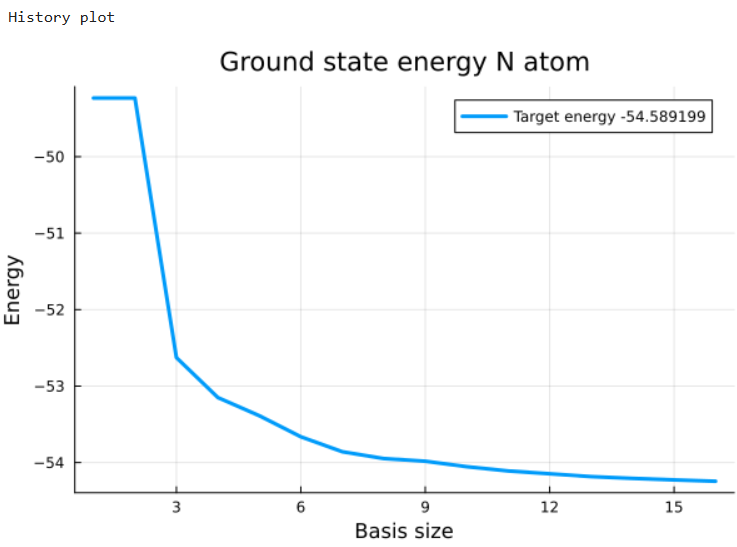
\includegraphics[width=0.72\textwidth]{fig_N_convergence.png}
\caption{Convergence of the $^{14}\mathrm{N}$ ${}^4S$ ground-state energy
(\texttt{N\_Pvec}) with basis size $K$ toward the target energy
$-54.589\,199$~a.u. The energy decreases monotonically as basis functions are
added; the value at $K=16$ ($-54.2445$~a.u.) remains above the reference because
of the short ($\sim$4-cycle) optimization used here (see text).}
\label{fig:Nconv}
\end{figure}}{}

% =====================================================================
\section{Conclusion}
\label{sec:conclusion}

We have presented an open, modular Julia implementation of the explicitly
correlated Gaussian method that covers real and complex $L=0$ Gaussians, the
$L=0$ nitrogen basis with a cubic angular prefactor, and $L=1$ Gaussians. The
implementation itself is the principal contribution: a reproducible JSON-driven
configuration system; a modular matrix-element architecture in which each
physical model sits behind a single uniform interface; an exact analytic energy
gradient generated by automatic differentiation (eliminating hand-coded
derivatives and the cost of finite differences); and an on-the-fly construction
of the permutational-symmetry operator from a human-readable Young-operator
string, together with a symmetry-term truncation/ramp scheme that concentrates
optimization effort on the dominant permutation terms. The correctness of the
code is established by reproducing published ground-state energies for
$\mathrm{HD^+}$, $\mathrm{D_3^+}$, $\mathrm{H_3^+}$, $^9\mathrm{Be}$, $\mathrm{He}$,
$^7\mathrm{Li}$, $^{14}\mathrm{N}$, and $\mathrm{Ps_2}$, and the text-file bridge
to \textsc{atom-mol-nonBO} allows independent cross-checks of the energies.

Future work includes a fuller parallelization of the symmetry-term sums over
the Hamiltonian, overlap and gradient matrix elements, and an evaluation of
batched/accelerator implementations of the matrix-element kernels for larger
basis sets, where the permutational sum dominates the cost.

\paragraph{Code availability.}
\texttt{ECG\_Julia} is released as open-source software, together with the JSON
configuration files that reproduce every entry of Table~\ref{tab:results}, so
that the results reported here can be regenerated and the implementation reused
and extended. \emph{[Repository URL and open-source license to be inserted on
release.]}

\paragraph{Acknowledgements.}
The author thanks Prof.\ Sergiy Bubin and Dr.\ Keeper L. Sharkey for the ECG methodology,
reference data and the \textsc{atom-mol-nonBO} program on which this
implementation builds.

% =====================================================================
\appendix

\section{Hamiltonian and permutational symmetry}
\label{app:ham}
(After Sharkey and Adamowicz~\cite{Sharkey2014}.)

For an $n$-electron atomic system with only $s$ electrons the basis function is
spherically symmetric and has the ECG form
\begin{equation}
\psi_f=\exp\!\left[-\rvec'(A_f\otimes I_3)\rvec\right],
\end{equation}
with $A_f$ an $n\times n$ symmetric matrix. The quadratic form
$\rvec'(A_f\otimes I_3)\rvec$ includes all one- and two-pseudoelectron
exponential couplings. For three $p$-electrons coupled to $L=0,\,M=0$ the
angular part is $(x_jy_i-x_iy_j)z_k+(x_iy_k-x_ky_i)z_j+(x_ky_j-x_jy_k)z_i$, and
the matrix elements are derived from the general cubic-prefactor ECG
$\phi_f=(\rvec'\mathbf{v}_f^x)(\rvec'\mathbf{v}_f^y)(\rvec'\mathbf{v}_f^z)\exp[-\rvec'\mathbf{A}_f\rvec]$.

The permutational symmetry is enforced by projecting each basis function with a
symmetry-projection operator $\Ycal$:
\begin{equation}
\psi_k=\Ycal\,\Phi_k=\sum_P \chi_P\, r_1^{m_k}\,
\exp\!\left[-\rvec'(\tau_P'L_kL_k'\tau_P\otimes I_3)\rvec\right].
\end{equation}
For $n$ fermions with total spin $s$, the symmetry quantum number is
$p=\tfrac{n}{2}-s$ and the partition $\mu=[2^p\,1^{n-2p}]$ defines the Young
tableau. For nitrogen ($^4S$, three $p$-electrons, $s=\tfrac32$,
$\mu=[2^2\,1^3]$) the projector is $\Ycal=\hat S\hat A$ with
$\hat S=(\hat 1+\hat P_{56})(\hat 1+\hat P_{78})$ and
\begin{equation}
\hat A=(\hat 1-\hat P_{68})(\hat 1-\hat P_{57})(\hat 1-\hat P_{27}-\hat P_{25})
(\hat 1-\hat P_{32}-\hat P_{37}-\hat P_{35})
(\hat 1-\hat P_{43}-\hat P_{42}-\hat P_{47}-\hat P_{45}),
\end{equation}
so that the complete operator $\hat P=\Ycal^{\dagger}\Ycal$ has
$n!=7!=5040$ terms.

\section{Solving the secular equation and the energy gradient}
\label{app:secular}
(After Bubin and Adamowicz~\cite{Bubin2008,Bubin2013}.)

With $\psi(\rvec)=\sum_k c_k\,\Ycal\,\phi_k(\rvec)$, minimizing the energy with
respect to the $c_k$ gives the generalized eigenproblem
$(\mathbf{H}-\varepsilon\mathbf{S})\mathbf{c}=0$ with Hermitian
$\mathbf{H},\mathbf{S}$. The nonlinear parameters are optimized with the energy
gradient
\begin{equation}
\frac{\partial\varepsilon}{\partial\alpha}
=\mathbf{c}^{\dagger}\!\left(\frac{\partial\mathbf{H}}{\partial\alpha}
-\varepsilon\frac{\partial\mathbf{S}}{\partial\alpha}\right)\mathbf{c},
\end{equation}
where $\alpha$ stacks the lower-triangular elements of all $L_k$.

\paragraph{Automatic differentiation of the molecular integrals.}
Rather than hand-coding $\partial\vech\mathbf{H}/\partial\alpha$ and
$\partial\vech\mathbf{S}/\partial\alpha$, the per-element derivatives are
obtained by forward-mode automatic differentiation~\cite{Revels2016}. The
type-generic matrix-element kernel propagates dual numbers through the matrix
build, determinant, inverse and $36$-term sum, so a single Jacobian of
$[\mathrm{H}_{kl},\mathrm{S}_{kl}]$ with respect to $\vech L_k$ yields
\begin{equation}
\mathrm{Dk}=\Big(\tfrac{\partial \mathrm{H}_{kl}}{\partial \vech L_k},\,
\tfrac{\partial \mathrm{S}_{kl}}{\partial \vech L_k}\Big),\qquad
\mathrm{Dl}=\Big(\tfrac{\partial \mathrm{H}_{kl}}{\partial \vech L_l},\,
\tfrac{\partial \mathrm{S}_{kl}}{\partial \vech L_l}\Big).
\end{equation}
For the complex module ($\mathbf{C}_k=\mathbf{A}_k-\mathrm{i}\mathbf{B}_k$) the
Jacobian of $[\operatorname{Re}\mathrm{H},\operatorname{Im}\mathrm{H},
\operatorname{Re}\mathrm{S},\operatorname{Im}\mathrm{S}]$ is recombined into the
complex $\mathrm{Dk},\mathrm{Dl}$.

\paragraph{Analytic gradient assembly.}
During optimization only the function $i$ being optimized varies, so
$\partial\mathbf{H}/\partial\alpha$ and $\partial\mathbf{S}/\partial\alpha$ are
non-zero only in row/column $i$. Working with the raw (unnormalized)
generalized eigenproblem $\mathbf{H}_r\mathbf{c}=E\,\mathbf{S}_r\mathbf{c}$ and
its $\mathbf{S}_r$-normalized ground eigenvector $\mathbf{c}$ (the eigenvalue is
invariant under the diagonal normalization), the gradient is
\begin{equation}
\frac{\partial E}{\partial \vech L_i}
=2\,\operatorname{Re}\!\Big[\overline{c_i}\sum_l c_l\,(g^H_l-E\,g^S_l)\Big],
\qquad
(g^H_l,g^S_l)=\sum_j \mathrm{YHYCoeff}[j]\,
\frac{\partial(\mathrm{H}_{il},\mathrm{S}_{il})}{\partial \vech L_i},
\end{equation}
which reduces, for real $\mathbf{c},\mathbf{H},\mathbf{S}$, to
$2\,c_i\sum_l c_l(g^H_l-E\,g^S_l)$. This is implemented as the type-generic
\texttt{loss\_grad!}\ and was verified against central finite differences to a
relative accuracy of $\sim10^{-7}$ for both the real and complex nitrogen
modules.

\section{The \texorpdfstring{$\vecop$}{vec} and \texorpdfstring{$\vech$}{vech} operators}
\label{app:vec}
(After Kinghorn~\cite{Kinghorn1996}.)

The $\vecop$ operator stacks the columns of an $n\times n$ matrix $A$ into an
$n^2$-vector. The half-vectorization $\vech A$ stacks the lower-triangular
elements into an $n(n+1)/2$-vector; e.g.\ for $n=3$,
\begin{equation}
\vech A=\big(a_{11},a_{21},a_{31},a_{22},a_{32},a_{33}\big)'.
\end{equation}
The nonlinear parameters of a basis function are the entries of $\vech L_k$.

\paragraph{Pvec.}
To avoid explicit multiplication by sparse permutation matrices, the
forward permutation $(Pv=v'P')$ is stored in the first half and the backward
permutation $(P'v=vP')$ in the second half of a $2n$-vector (Pvec). A permuted
matrix element is then obtained by an index gather,
$ (PAP')_{(s,t)}=A_{(\mathrm{pvec}(s),\mathrm{pvec}(t))}$ and
$ (P'AP)_{(s,t)}=A_{(\mathrm{pvec}(s+n),\mathrm{pvec}(t+n))}$,
which is where the nitrogen \texttt{Pvec} kernels save operations.

% =====================================================================
\begin{thebibliography}{99}

\bibitem{Bubin2013}
S.\ Bubin, M.\ Pavanello, W.-C.\ Tung, K.\ L.\ Sharkey, and L.\ Adamowicz,
\emph{Born--Oppenheimer and Non-Born--Oppenheimer, Atomic and Molecular
Calculations with Explicitly Correlated Gaussians}, Chem.\ Rev.\ \textbf{113},
36--79 (2013). \href{https://doi.org/10.1021/cr200419d}{doi:10.1021/cr200419d}.

\bibitem{Sharkey2014}
K.\ L.\ Sharkey and L.\ Adamowicz, \emph{An algorithm for nonrelativistic
quantum-mechanical finite-nuclear-mass variational calculations of nitrogen
atom in $L=0$, $M=0$ states using all-electron explicitly correlated Gaussian
basis functions}, J.\ Chem.\ Phys.\ \textbf{140}, 174112 (2014).
\href{https://doi.org/10.1063/1.4873916}{doi:10.1063/1.4873916}.

\bibitem{Bubin2008}
S.\ Bubin and L.\ Adamowicz, \emph{Energy and energy gradient matrix elements
with $N$-particle explicitly correlated complex Gaussian basis functions with
$L=1$}, J.\ Chem.\ Phys.\ \textbf{128}, 114107 (2008).
\href{https://doi.org/10.1063/1.2894866}{doi:10.1063/1.2894866}.

\bibitem{Kinghorn1996}
D.\ B.\ Kinghorn, \emph{Integrals and Derivatives for Correlated Gaussian
Functions Using Matrix Differential Calculus}, Int.\ J.\ Quantum Chem.\
\textbf{57}, 141--155 (1996).

\bibitem{Hornyak2019}
I.\ Horny\'ak, L.\ Adamowicz, and S.\ Bubin, \emph{Ground and excited $^1S$
states of the beryllium atom}, Phys.\ Rev.\ A \textbf{100}, 032504 (2019).

\bibitem{Bralin2019}
A.\ Bralin, S.\ Bubin \emph{et al.}, \emph{The Rydberg series of the lithium
atom: calculations with all-electron explicitly correlated Gaussian functions},
Chem.\ Phys.\ Lett.\ \textbf{730}, 497--502 (2019).
\href{https://doi.org/10.1016/j.cplett.2019.06.051}{doi:10.1016/j.cplett.2019.06.051}.

\bibitem{Seth2011}
P.\ Seth, P.\ L.\ R\'ios, and R.\ J.\ Needs, J.\ Chem.\ Phys.\ \textbf{134},
084105 (2011).

\bibitem{Pavanello2009}
M.\ Pavanello and L.\ Adamowicz, \emph{High-accuracy calculations of the
ground, $1\,{}^1A_1'$, and the $2\,{}^1A_1'$, $2\,{}^3A_1'$, and $1\,{}^1E'$
excited states of $\mathrm{H_3^+}$}, J.\ Chem.\ Phys.\ \textbf{130}, 034104
(2009). \href{https://doi.org/10.1063/1.3058634}{doi:10.1063/1.3058634}.

\bibitem{Lang2024}
L.\ Lang, H.\ M.\ Cezar, L.\ Adamowicz, and T.\ B.\ Pedersen, \emph{Quantum
Definition of Molecular Structure}, J.\ Am.\ Chem.\ Soc.\ \textbf{146}(3),
1760--1764 (2024). \href{https://doi.org/10.1021/jacs.3c11467}{doi:10.1021/jacs.3c11467}.

\bibitem{ATOMMOLnonBO}
S.\ Bubin and L.\ Adamowicz, \emph{Computer program \textup{\textsc{atom-mol-nonBO}}
for performing calculations of ground and excited states of atoms and molecules
without assuming the Born--Oppenheimer approximation using all-particle complex
explicitly correlated Gaussian functions}, J.\ Chem.\ Phys.\ \textbf{152},
204102 (2020). \href{https://doi.org/10.1063/1.5144268}{doi:10.1063/1.5144268}.
GitHub: \url{https://github.com/sbubin/ATOM-MOL-nonBO}.

\bibitem{Revels2016}
J.\ Revels, M.\ Lubin, and T.\ Papamarkou, \emph{Forward-Mode Automatic
Differentiation in Julia}, arXiv:1607.07892 (2016).

\bibitem{Bezanson2017}
J.\ Bezanson, A.\ Edelman, S.\ Karpinski, and V.\ B.\ Shah, \emph{Julia: A Fresh
Approach to Numerical Computing}, SIAM Rev.\ \textbf{59}(1), 65--98 (2017).

\bibitem{HeliumAtom}
Reference $1{}^1S$ ground-state energy of helium (finite mass), as used in the
\texttt{He\_CGL0} notebook; cf.\ the helium-atom data, \emph{Wikipedia: Helium atom}.

\end{thebibliography}

\end{document}
